\documentclass[12pt]{scrartcl}
\usepackage[ngerman]{babel}


\usepackage{amsmath, amssymb}

\usepackage{array}  % for the tables

\usepackage{nameref}  % for referencing with name

\usepackage{hyperref}  % for hyperlinks

\usepackage{pgfplots}

\usepackage{mathrsfs}

\usepackage{graphicx}  % for the images

\usepackage{glossaries}

\usepackage{xcolor, colortbl}

\pgfplotsset{compat=1.15}  % for the graphs

\usetikzlibrary{arrows} % for the graphs

\definecolor{Gray}{gray}{0.85}

% hyperlinks
\hypersetup{
    colorlinks,
    citecolor=black,
    filecolor=black,
    linkcolor=black,
    urlcolor=black
}

\bibliographystyle{IEEetran}

\author{David Jäggli}

\title{Analysis Differenzialrechnung}

\begin{document}

\maketitle

\tableofcontents

\newpage


\section{Ableitung} 
\subsection{Ziele der Ableitungen}

Die folgenden drei Punkte werden mittels einer Differenzialrechnung erreicht.

\begin{enumerate}
    \item Das Bestimmen der Tangente in einem Punkt der Kurve $y=f(x)$
    \item Das Linearisieren einer Funktion $y=f(x)$ (siehe Kapitel \ref{approximation})
    \item Mit einer neuen Funktion $f'(x)$ (1. Ableitung von $f(x)$ die Steigung an jedem Punkt $x$ von der ursprünglichen Funktion $f(x)$ zu ermitteln.
    \item Mit einer neuen Funktion $f''(x)$ (2. Ableitung von $f(x)$) zu bestimmen, ob sich die ursprüngliche Funktion $f(x)$ an jeder beliebigen Stelle $x$ in einer Links- resp. Rechtskrümmung befindet
\end{enumerate}


\section{Differenzierbarkeit}
Eine Funktion ist immer dann differenzierbar, wenn sie stetig ist und keinen Knick 
hat.

\subsection{Regeln}
\subsubsection{Potenzregeln}

\renewcommand{\arraystretch}{1.5}
\begin{center}
    \begin{tabular}{ | m{10em} | m{10em} | m{10em} | }
        \hline
        Ursprungsfunktion & Ableitung & Beispiel \\ 
        \hline
        $f(x) = x^n$ & $f'(x) = n \cdot x^{(n-1)} $ & $x^2 \Rightarrow 2x$\\ 
        \hline
        $f(x) = c = 2$ (konst.) & $f'(x) = 0$ & $5 \Rightarrow 0$ \\
        \hline
        $f(x) = e^x$ & $f'(x) = e^x$ & $e^x \Rightarrow e^x$ \\
        \hline
        $f(x) = a^x$ & $f'(x) = ln(a) \cdot a^x$ & $5^x \Rightarrow ln(5) \cdot 5^x$ \\
        \hline
        $f(x) = ln(x)$ & $f'(x) = \frac{1}{x}$ & $ln(x) \Rightarrow \frac{1}{x}$ \\
        \hline 
        $f(x) = \frac{a}{(x + n)} $ & $ f'(x) = -\frac{a}{(x+n)^2} $ & $\frac{500}{x + 5} \Rightarrow -\frac{500}{(x+5)^2}$\\
        \hline 
        $f(x) = log_a(x) $ & $f'(x) = \frac{1}{x \cdot ln(a)}$ & $log_3(x) \Rightarrow \frac{1}{x * ln(3)}$ \\
        \hline 

    \end{tabular}
\end{center}

% -------- begin of chain rules ----------------
\newpage

\subsubsection{Weiterführende Regeln}

\begin{center}
\textbf{Faktorregel \& Beispiel:} 
\[ f(x) = a \cdot g(x) = a \cdot g'(x)\]
\[f(x)=2 \cdot x^3 \Rightarrow f'(x)=2 \cdot (x^3)' = 2 \cdot 3 \cdot x^2 = \underline{6x^2}\]

\newpage
\textbf{Summenregel \& Beispiel:} 
\[ (f(x) + g(x))' = f'(x) + g'(x) \]
\[ x^2 + x^3 \Rightarrow \underline{2x + 3x^2}\]

\hspace{0pt} \\
\hspace{0pt} \\
\noindent
\textbf{Produktregel \& Beispiel:} 
\[ (f(x) \cdot g(x))' =  f'(x) \cdot g(x) + f(x) \cdot g'(x)\]
\[x^3 \cdot x^3 \Rightarrow 3x^2 \cdot x^3 + x^3 \cdot 3x^2 = 3x^5 + 3x^5 = \underline{6x^5}\]


\hspace{0pt} \\
\hspace{0pt} \\
\noindent
\textbf{Quotientenregel \& Beispiel:} 
\[\left(\frac{f(x)}{g(x)}\right)' = \frac{f'(x) \cdot g(x) - f(x) \cdot g'(x)}{(g(x))^2}\]
\[f(x)= \frac{e^x}{x^2} \Rightarrow f'(x) = \frac{e^x}{(2x)^2} = \frac{20x^5 - 4x^5}{4x^2} = \frac{16x^5}{4x^2} = \underline{4x^3}\]

\hspace{0pt} \\
\hspace{0pt} \\
\noindent
\textbf{Kettenregel \& Beispiel:} 
\[f(g(x)) \Rightarrow (f(g(x)))' = f'(g(x)) \cdot g'(x)\]
\[f(x) = ln(x^4) = ln(g(x)) \Rightarrow f'(x) = \frac{1}{g(x)} \cdot g'(x) \Rightarrow \frac{4x^3}{x^4} = \frac{4}{x}\]


\end{center}

% ------ End of chain rules ----------
\newpage

\section{Tangente \& Normale}
\subsection{Tangente einer Funktion}
Die Tangente an einem Punkt $x_0$ in einer Funktion lautet folgendermassen:\\
$ f'(x_0) \cdot (x - x_0) + y_0$ wobei $y_0 = f(x_0)$\\

\noindent
Der Winkel einer Geraden (Tangente) zur x-Achse kann mit der Tangens resp. Arcustangens 
Funktion berechnet werden: $\alpha = arctan(f'(x_0)) \rightarrow$ an der Stelle 
$x_0$ hat die Tangente einen Winkel von $\alpha$ zur x-Achse.


\subsection{Normale}
Die Normale oder senkrechte Funktion lässt sich folgendermassen berechnen:\\
Aus  $g_1 \perp g_2  $ folgt, dass $m_1 \cdot m_2 = -1$ \\ 
resp. $m_1 = -\frac{1}{m_2}$ \\
\\ 
\noindent
Eine Gerade ist definiert durch: $y = mx + q$. Die Steigung $m$ der Normalen ist wie oben
beschrieben einfach der negative Kehrwert der Steigung der Tangente. Den $y$-Wert 
kann man durch Einsetzen des Punktes berechnen. \\

\noindent
\underline{\textbf{Beispiel:}} \\
Gegeben: $f(x) = x^2 -2x + 1$ \\ %\quad \Rightarrow \quad f'(x) = 2x -2$\\%
Gesucht: Tangente und Normale bei $x=0$\\
Steigung der Tangente: $m_1 = f'(x=0) = -2$ \\
Steigung der Normale: $m_2 = -\frac{1}{m_1} = 0.5$ \\
\\
Für q einfach die Steigung in der Gleichung einsetzen.\\
Durch $f(x)$ ist definiert, dass bei $x=0 \rightarrow y=1$, heisst:\\
Für die Tangente: $1 = m_1x + q \Rightarrow 1= -2x + q \Rightarrow q = 1$ weil $x=0$\\
Für die Normale: $1 = m_2x + q \Rightarrow 1= 0.5x + q \Rightarrow q = 1$ weil $x=0$\\
\\
\noindent
Tangente = \underline{$f(x) = -2x + 1$}\\
Normale = \underline{$f(x) = 0.5x + 1$}\\

\newpage
\section{Annäherungen} \label{approximation}
Oftmals ist es nicht nötig (zu aufwändig/schwierig) oder gar nicht möglich die exakte 
Funktion zu berechnen (z.B. ln(x)). Um dieses Problem zu beheben, erstellt man eine Annäherungsfunktion
in einem gewissen Bereich, welche genügend nah an die ursprüngliche Funktion herankommt.

\subsection{Lineare Approximation}

Eine lineare Annäherung an einem Punkt $x_0$ ist die Tangente der 
Funktion am Punkt $x_0$, welche mit der Tangentenformel berechnet werden kann:

\[ \frac{f'( x_0 )}{1!} ( x - x_0) \Rightarrow f'( x_0 ) ( x - x_0) \] 


\subsection{Höhere Approximation (Taylorpolynom)}

Eine quadratische oder kubische Annäherung (Taylorpolynom) einer Funktion kommt viel näher an die tatsächliche Funktion heran, 
da sie die Krümmung berücksichtigt. Sofern die Ursprungsfunktion $f(x)$ n-mal
differenzierbar ist, kann ein Taylorpolynom wie folgt gebildet werden:
\[
    \frac{f^{(n)} ( x_0 )}{n!} ( x - x_0)^n +
    \frac{f^{(n-1)} ( x_0 )}{(n - 1)!} ( x - x_0)^{n - 1} + .... +
    \frac{f'' ( x_0 )}{2!} ( x - x_0)^2 + 
    f' ( x_0 ) ( x - x_0) + f(x_0)
\]


\newcommand{\drawmisding}{
    % \begin{tikzpicture}[line cap=round,line join=round,>=triangle 45,x=1cm,y=1cm]
    %     \begin{axis}[
    %         x=1cm,y=1cm,
    %         axis lines=middle,
    %         ymajorgrids=true,
    %         xmajorgrids=true,
    %         xmin=-7,
    %         xmax=7,
    %         ymin=-2,
    %         ymax=11,
    %         xtick={-12,-11,...,18},
    %         ytick={-7,-6,...,11},]
    %         \clip(-12.34,-7.36) rectangle (18.3,11.92);
    %         \draw [samples=50,rotate around={0:(0,0)},xshift=0cm,yshift=0cm,line width=2pt,domain=-7:7)] plot (\x,{(\x)^2/2/0.5});
    %         \begin{scriptsize}
    %         \draw[color=black] (-0.54,1.23) node {$f$};
    %         \end{scriptsize}
    %     \end{axis}
    % \end{tikzpicture}
    \begin{tikzpicture}[line cap=round,line join=round,>=triangle 45,x=1cm,y=1cm]
        \clip(-2,-3) rectangle (2,3);
        \draw[line width=2pt,smooth,samples=200,domain=0.14:2.5] plot(\x,{ln((\x))});
        \begin{scriptsize}
            \draw[color=black] (0,-4) node {$f$};
        \end{scriptsize}
    \end{tikzpicture}
}

\newpage

\section{Die Monotonie und Krümmung}
Ob eine Funktion $f(x)$ am Punk $x_0$ links oder rechtsgekrümmt ist, kann man mit der 2. 
Ableitung bestimmen. \\
$f''(x) > 0 \Rightarrow$ \textbf{linksgekrümmt/konvex}\\
$f''(x) < 0 \Rightarrow$ \textbf{rechtsgekrümmt/konkav}\\
$f''(x) = 0 \Rightarrow$ \textbf{Wendepunkt}

\renewcommand{\arraystretch}{1.5}
\begin{center}
    \begin{tabular}{ | p{5em} | p{14em} | b{14em} | }
        \hline
         & $f'(x) > 0 \Rightarrow$ wachsend & $f'(x) < 0 \Rightarrow$ fallend\\ 
        \hline
        $f''(x) > 0$ konvex & 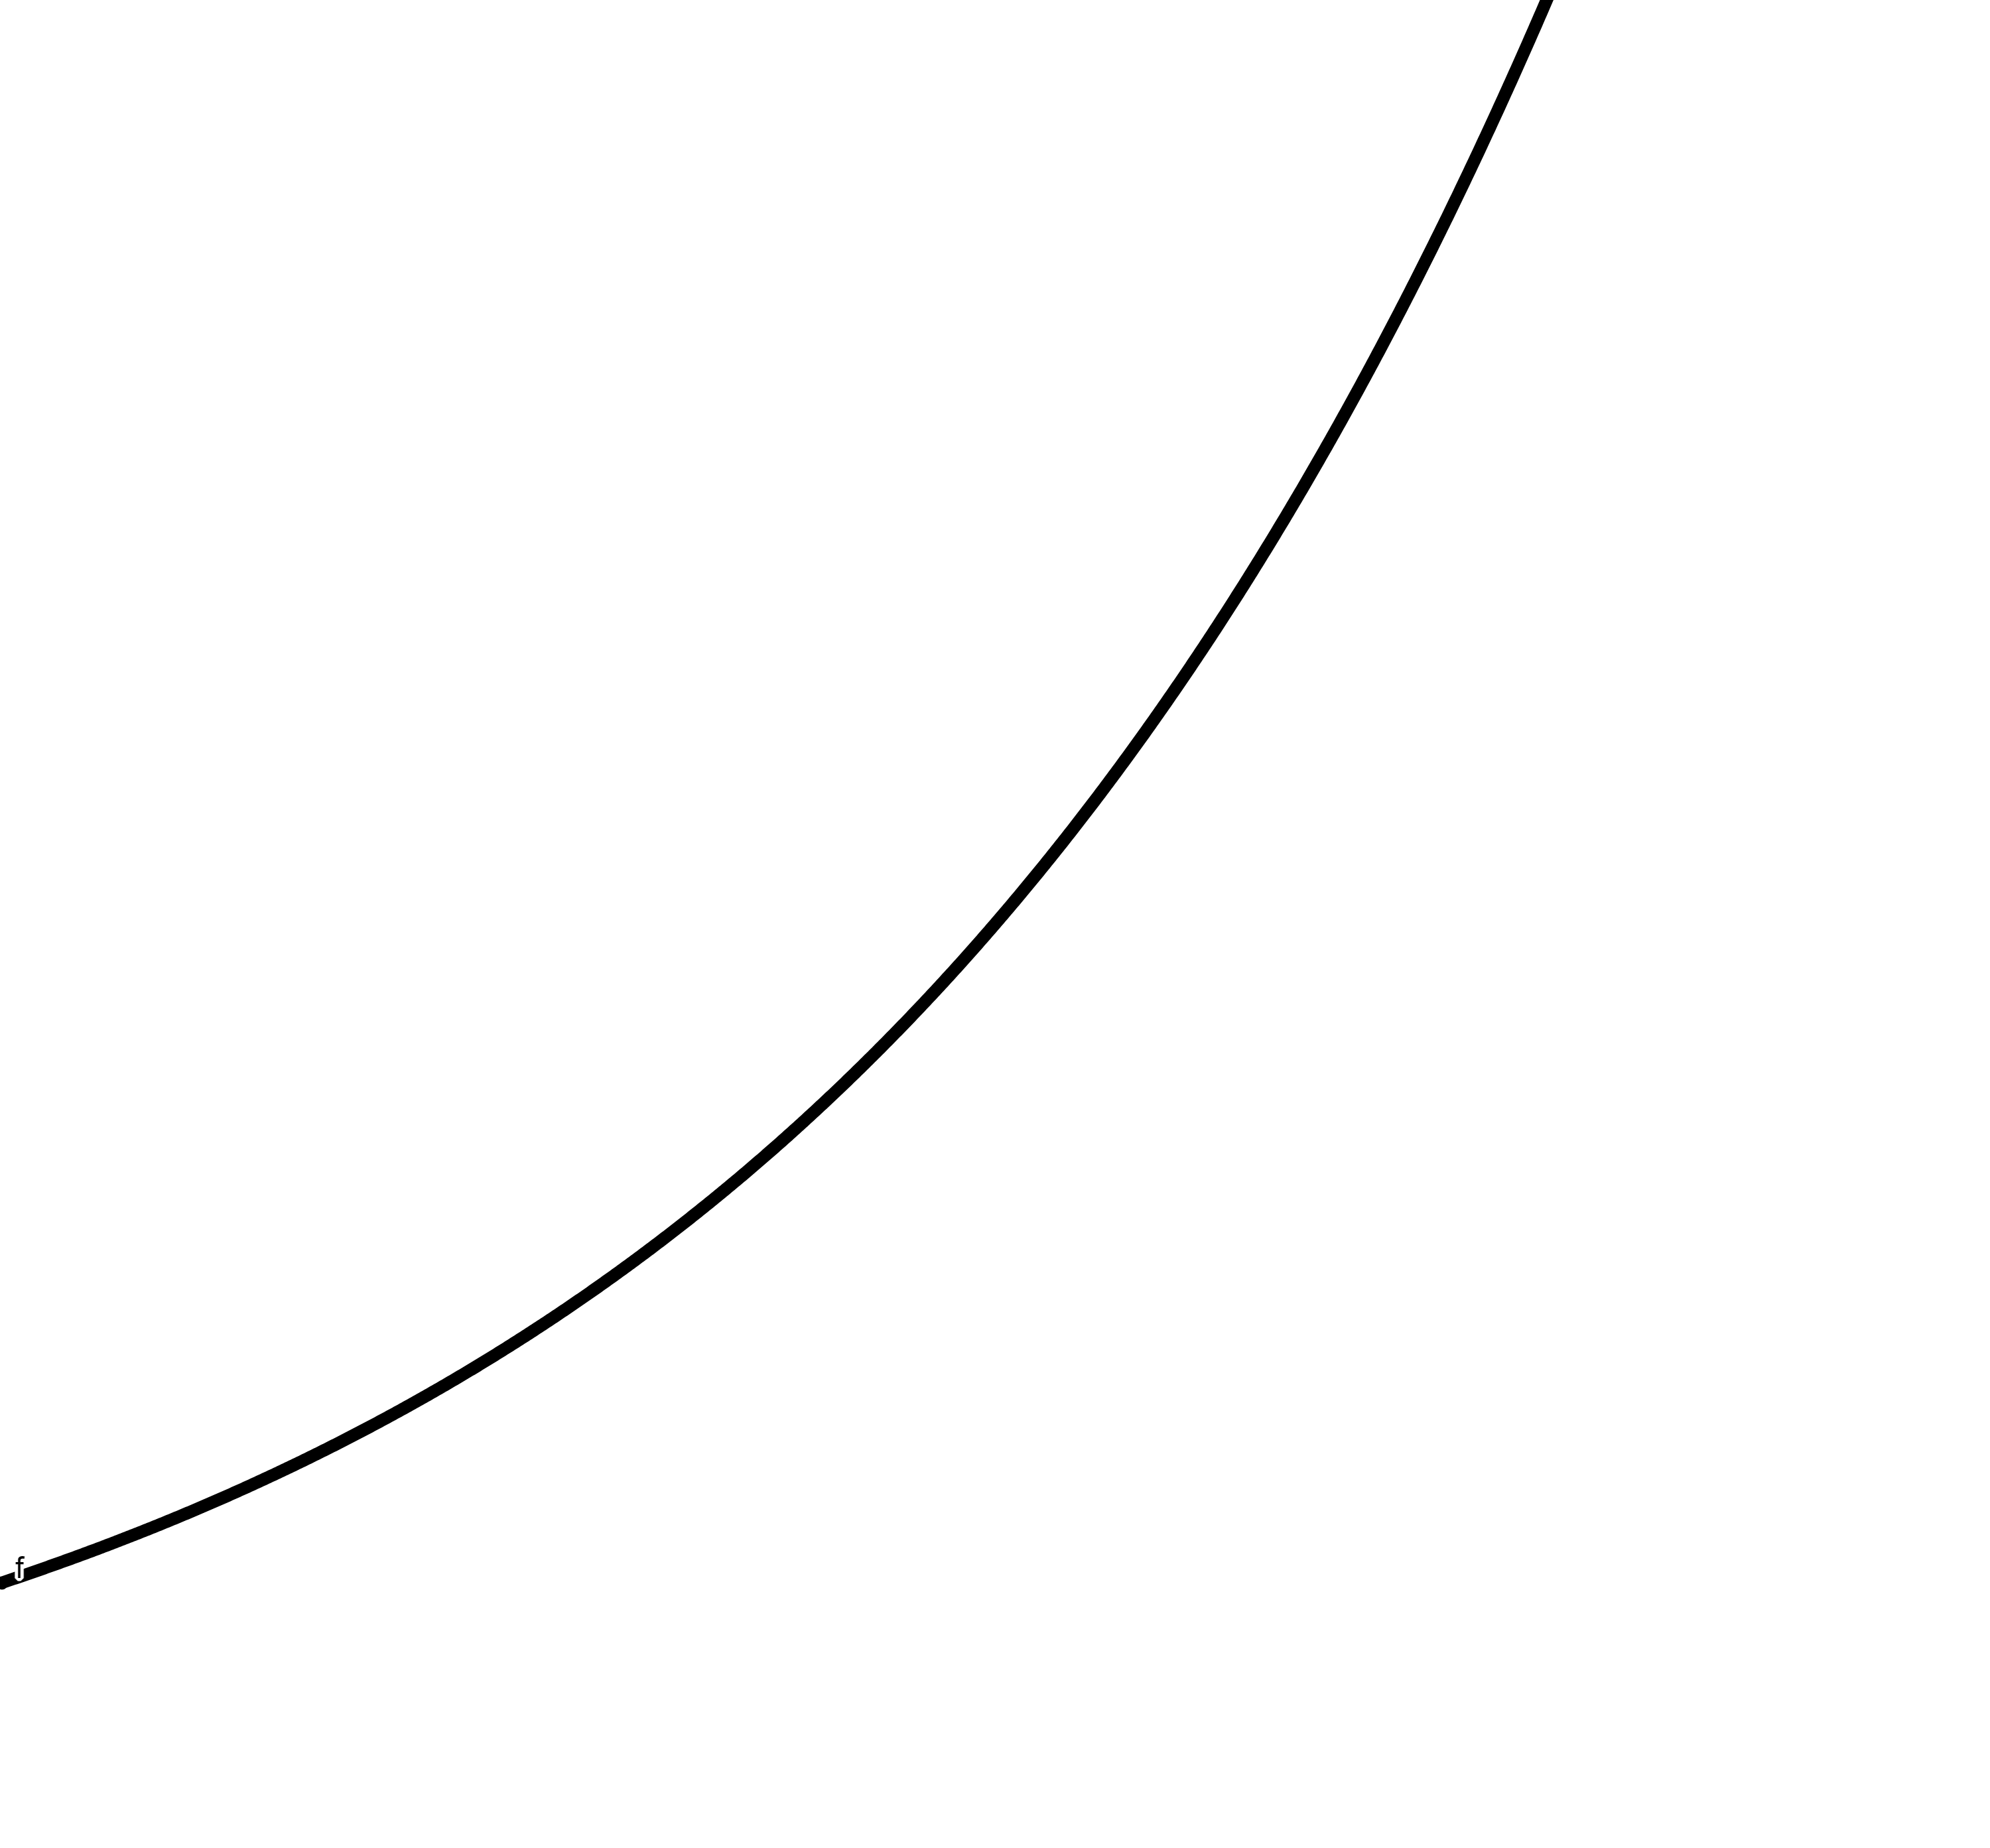
\includegraphics[width=3cm]{img/rising_convex.png} & \drawmisding\\ 
        \hline
        $f''(x) < 0$ konkav & &\\ 
        \hline
    \end{tabular}
\end{center}


\newpage
\section{Kurvendiskussion}

\subsection{Berechnungen ohne Differenzialrechnung}
\begin{center}
    \begin{tabular}{| p{13em} | p{23em} | }
        \hline
        \rowcolor{Gray}
        \textbf{Eigenschaft}            & \textbf{Mathematische Bedingung} \\
        \hline
        Schnittpunkt mit der y-Achse    & Die Funktion $y=f(x)$ an $x=0$ resp. $f(0)$ ausrechnen $\Rightarrow$ $P=(0, f(x))$ \\
        \hline
        Nullstellen                     & Lösung der Gleichung $f(x)=0$. \\
        \hline
        Vertikale Asymptote (ein Pol)   & In diesem Fall lautet die Gleichung \newline $y = f(x) = \frac{g(x)}{h(x)}$ und beim Pol ist $h(x)=0$\\
        \hline
        Symmetrien (gerade resp. ungerade Funktionen) & Für \textbf{gerade} Funktionen $f(x) = f(-x)$ \newline Für \textbf{ungerade} Funktionen $f(x) = -f(-x)$ \newline \quad \quad \quad resp. $-f(x) = f(-x)$ \\
        \hline
    \end{tabular}
\end{center}

\subsection{Lokale Extremwerte}
\subsubsection{Extremalwert}
Ein Extremalwert ist immer dort, wo keine Steigung herrscht, also $f'(x) = 0$ \\
Ein Minimalwert ist bei einer Linkskurve, also $f''(x) > 0$. Und ein Maximalwert
bei einer Rechtskurve, also $f''(x) < 0$.

\begin{center}
    \begin{tabular}{|p{7em}|p{9em}|p{18em}|}
        \hline
        \rowcolor{Gray}
        \textbf{Eigenschaft} & \textbf{99 \% Regel} & \textbf{100 \% resp. Ausnahmeregel}\\
        \hline
        Generel: & $f'(x_0) = 0$ & $f'(x_0) = f''(x_0) \dots f^{(n - 1)}(x_0) = 0$\\
        \hline
        Maximum: & $f''(x_0) < 0$ & für n gerade ist $f^{(n)}(x_0) < 0$\\
        \hline
        Minimum: & $f''(x_0) > 0$ & für n gerade ist $f^{(n)}(x_0) > 0$\\
        \hline
    \end{tabular}
\end{center}

\subsubsection{Wendepunkte}
Ein Wendepunkt ist dort wo die Kurve keine Krümmung hat, also $f''(x) = 0$.
\begin{center}
    \begin{tabular}{|p{7em}|p{9em}|p{18em}|}
        \hline
        \rowcolor{Gray}
        \textbf{Eigenschaft} & \textbf{99 \% Regel} & \textbf{100 \% resp. Ausnahmeregel}\\
        \hline
        Generel: & $f''(x_0) = 0$ & $f''(x_0) = \dots f^{(n - 1)}(x_0) = 0$\\
        \hline
        Zusätzlich: & $f'''(x_0) \neq 0$ & für n ungerade ist $f^{(n)}(x_0) \neq 0$\\
        \hline
    \end{tabular}
\end{center}

\subsubsection{Terrassenpunkte}
Ein Terrassenpunkt ist ein Wendepunkt mit horizontaler Tangente an der Stelle $x_0$.
\begin{center}
    \begin{tabular}{|p{7em}|p{9em}|p{18em}|}
        \hline
        \rowcolor{Gray}
        \textbf{Eigenschaft} & \textbf{99 \% Regel} & \textbf{100 \% resp. Ausnahmeregel}\\
        \hline
        Generel: & $f'(x_0) = f''(x_0) = 0$ & $f'(x_0) = f''(x_0) \dots f^{(n - 1)}(x_0) = 0$\\
        \hline
        Zusätzlich: & $f'''(x_0) \neq 0$ & für n ungerade ist $f^{(n)}(x_0) \neq 0$\\
        \hline
    \end{tabular}
\end{center}


% \bibliography{quantum_ready}

\end{document}